\section{Un primer programa}

\begin{frame}{Hola}
\begin{columns}

\column{ .5\textwidth}
\begin{block}{hola.cpp}
\lstinputlisting{02-hola/hola/hola.cpp}
\end{block}

\column{.5\textwidth}
  \begin{itemize}
    \item Archivo de cabecera: \mode<presentation>{\cppid{iostream}.}
      \mode<article>{
        \begin{itemize}
          \item Se sigue el paradigma de sustitución de texto.
        \end{itemize}
      }
    \item Importación de espacio de nombres: \mode<presentation>{\cppid{std}.}
      \mode<article>{
        \begin{itemize}
          \item Alcance que contiene elementos de una biblioteca para evitar conflictos de nombrado.
          \item Es distinto de los modelos de \emph{paquetes} de otros lenguajes.
        \end{itemize}
      }
    \item Programa principal: \mode<presentation>{\cppid{main}.}
      \mode<article>{
        \begin{itemize}
          \item Es el punto de entrada al programa.
          \item Hay cosas que ocurren antes.
          \item Hay cosas que ocurren después.
        \end{itemize}
      }
    \item Flujo de salida estándar: \mode<presentation>{\cppid{cout}.}
      \mode<article>{
        \begin{itemize}
          \item Es una variable global.
        \end{itemize}
      }
    \item Operador de salida: \mode<presentation>{\cppkey{<{}<}.}
      \mode<article>{
        \begin{itemize}
          \item Operador para enviar datos a la salida estándar.
          \item Definido para la mayoría de los tipos.
        \end{itemize}
      }
    \item Salto de línea: \mode<presentation>{\cppid{endl}.}
      \mode<article>{
        \begin{itemize}
          \item Equivalente a \cppid{"\\endl"}.
        \end{itemize}
      }
    \item Código de salida: \mode<presentation>{\cppid{0}.}
      \mode<article>{
        \begin{itemize}
          \item Devuleto al sistema operativo.
        \end{itemize}
      }
  \end{itemize}

\end{columns}
\end{frame}

\subsection{Compilación y enlace}

\begin{frame}[t]{Fases de la traducción}
\begin{itemize}
  \item Preprocesado:
    \begin{itemize}
      \item Procesa las directivas del compilador de una unidad de traducción.
    \end{itemize}
  \vfill
  \item Compilación:
    \begin{itemize}
      \item Traduce el código fuente a código ensamblador.
    \end{itemize}
  \vfill
  \item Ensamblado:
    \begin{itemize}
      \item Ensambla a código objeto.
      \item Normalmente integrada con compilación.
    \end{itemize}
  \vfill
  \item Enlazado:
    \begin{itemize}
      \item Resuelve referencias externas entre módulos objeto.
    \end{itemize}
\end{itemize}
\end{frame}

\begin{frame}[fragile]{El preprocesador}
\begin{columns}

\column{.5\textwidth}
\begin{tikzpicture}
\tikzset{
    archfuente/.style={rectangle,rounded corners,draw=black, top color=white, bottom color=blue!50,very thick, inner sep=0.5em, minimum size=0, text centered, font=\tiny},
    flecha/.style={->, >=latex', shorten >=1pt, thick},
    etiqueta/.style={text centered, font=\tiny} 
}  
\node[archfuente] (cab1) {arch1};
\node[right=1cm of cab1] (cab2) {...};
\node[archfuente, right=1cm of cab2] (cab3) {archN};
\node[archfuente, below =1cm of cab2] (iostream) {\cppid{iostream}};
\draw[flecha] (iostream) -- (cab1);
\draw[flecha] (iostream) -- (cab2);
\draw[flecha] (iostream) -- (cab3);
\node[etiqueta, below =0.1cm of cab1] {\emph{include}};
\node[etiqueta, below left =0.25cm and -0.3cm of cab2] {\emph{include}};
\node[etiqueta, below =0.1cm of cab3] {\emph{include}};
\node[archfuente, below=1cm of iostream] (holacpp) {\cppid{hola.cpp}};
\draw[flecha] (holacpp) -- (iostream);
\node[etiqueta,below left=0.1cm and -0.6cm of iostream] {\emph{include}};
\end{tikzpicture}

\pause
\column{.5\textwidth}
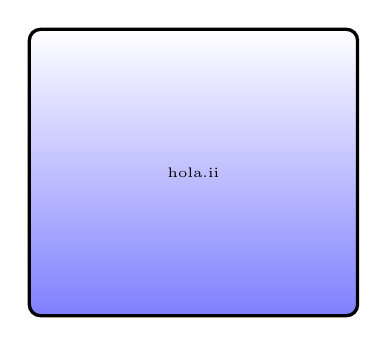
\begin{tikzpicture}
\tikzset{
    archfuente/.style={rectangle,rounded corners,draw=black, top color=white, bottom color=blue!50,very thick, inner sep=5em, minimum size=0, text centered, font=\tiny},
}  
\node[archfuente] () {hola.ii};
\end{tikzpicture}

\end{columns}
\begin{lstlisting}[style=terminal]
g++ hola.cpp -E -o hola.ii
\end{lstlisting}
\begin{itemize}
  \item 17524 líneas.
\end{itemize}
\end{frame}

\begin{frame}[fragile]{Compilación y ensamblado}
\begin{itemize}
\item \alert{Ensamblado}: Genera código ensamblador de una unidad de traducción.
  \begin{itemize}
    \item Es necesario ensamblar el código para llegar a código objeto
\begin{lstlisting}[style=terminal]
g++ hola.cpp -S -o hola.s
\end{lstlisting}
    \item 83 líneas.
  \end{itemize}
\item \pause \alert{Compilación}:Traduce a código objeto.
  \begin{itemize}
    \item Genera ensamblador.
    \item Ensambla a código ejecutable binario.
    \item Dejar sin resolver referencias externas.
  \end{itemize}
\begin{lstlisting}[style=terminal]
g++ hola.cpp -c -o hola.o
\end{lstlisting}
\end{itemize}
\end{frame}

\begin{frame}{Código ensamblador}
\begin{block}{hola.s}
\ldots
\mode<presentation>{
\lstinputlisting[language={[x86masm]Assembler},basicstyle=\tiny\ttfamily,firstline=10,lastline=28]{02-hola/hola/hola.s}
}
\mode<article>{
\lstinputlisting[language={[x86masm]Assembler},basicstyle=\ttfamily,firstline=10,lastline=28]{02-hola/hola/hola.s}
}
\ldots
\end{block}
\end{frame}

\begin{frame}[fragile]{Ensamblado}
\begin{itemize}
\item \pause Herramientas:
  \begin{itemize}
    \item Lista de símbolos de un archivo objeto:
\begin{lstlisting}[style=terminal]
nm hola.o
\end{lstlisting}
    \item \pause Código ensamblador de secciones ejecutables.
\begin{lstlisting}[style=terminal]
objdump -d hola.o
\end{lstlisting}
    \item \pause Información sobre las secciones del módulo objeto.
\begin{lstlisting}[style=terminal]
readelf -all hola.o
\end{lstlisting}
    \item \pause Si se quiere descifrar los nombres C++, se usa \verb-c++filt-.
\begin{lstlisting}[style=terminal]
nm hola.o | c++filt
\end{lstlisting}
  \end{itemize}
\end{itemize}
\end{frame}

\begin{frame}{Símbolos}
\begin{block}{nm hola.o}
\lstinputlisting[style=terminal,basicstyle=\tiny\ttfamily]{02-hola/hola/hola.nm}
\end{block}
\end{frame}

\begin{frame}{Símbolos con nombres descrifrados}
\begin{block}{nm hola.o | c++filt}
\lstinputlisting[style=terminal,basicstyle=\tiny\ttfamily]{02-hola/hola/hola.nm.cpp}
\end{block}
\end{frame}

\begin{frame}{Enlace}
\begin{itemize}
\item Resuelve referencias externas entre módulos objeto.
\item Genera programa ejecutable.
\end{itemize}
\begin{tikzpicture}
\tikzset{
    archfuente/.style={rectangle,rounded corners,draw=black, top color=white, bottom color=blue!50,very thick, inner sep=0.5em, minimum size=0, text centered, font=\tiny},
    flecha/.style={->, >=latex', shorten >=1pt, thick},
    etiqueta/.style={text centered, font=\tiny} 
}  
\node[archfuente] (cab1) {arch1};
\node[right=1cm of cab1] (cab2) {...};
\node[archfuente, right=1cm of cab2] (cab3) {archN};
\node[archfuente, below =1cm of cab2] (iostream) {\cppid{iostream}};
\draw[flecha] (iostream) -- (cab1);
\draw[flecha] (iostream) -- (cab2);
\draw[flecha] (iostream) -- (cab3);
\node[etiqueta, below =0.1cm of cab1] {\emph{include}};
\node[etiqueta, below left =0.25cm and -0.3cm of cab2] {\emph{include}};
\node[etiqueta, below =0.1cm of cab3] {\emph{include}};
\node[archfuente, below=1cm of iostream] (holacpp) {\cppid{hola.cpp}};
\draw[flecha] (holacpp) -- (iostream);
\node[etiqueta,below left=0.1cm and -0.6cm of iostream] {\emph{include}};
\node[archfuente,right=2cm of iostream] (holao) {\cppid{hola.o}};
\node[etiqueta,right=0.1cm of holao] {\emph{enlace}};
\draw[flecha] (holacpp) -- (holao);
\node[etiqueta,above right=0.1cm and 0.6cm of holacpp] {\emph{compilación}};
\node[archfuente,right=2cm of holacpp] (stdlib) {\cppid{libstdc++}};
\node[etiqueta,right=0.1cm of stdlib] {\emph{enlace}};
\node[archfuente,below right=0.5cm and 1cm of holao] (hola) {\cppid{hola}};
\draw[flecha] (holao) -- (hola);
\draw[flecha] (stdlib) -- (hola);
\end{tikzpicture}
\end{frame}

\subsection{Entornos de programación}

\begin{frame}[t]{Línea de comandos versus entornos integrados}
\begin{itemize}
  \item Línea de comandos:
    \begin{itemize}
      \item Editor para la edición de archivos fuentes (\emph{vim/gvim}, \emph{gedit}, \emph{emacs}, \ldots).
      \item Compilador (\textmark{\emph{g++}}, \emph{clang}, \ldots).
      \item Depurador.
      \item \ldots
    \end{itemize}
  \vfill
  \item Entornos integrados:
    \begin{itemize}
      \item Eclipse/CDT.
      \item Code::Blocks.
      \item KDevelop.
      \item Visual Studio.
      \item \textmark{CLion}.
    \end{itemize}
\end{itemize}
\end{frame}
